\documentclass[margin=5mm]{standalone}
\usepackage{tikz}
\usepackage{pxfonts}
\usepackage{enumitem}

\usetikzlibrary{calc,fit}


\makeatletter
% Default value for /my/box options
\def\my@boxoptions{}


\pgfkeys{
  /my/.cd,
  id/.store in=\my@id,
  name/.store in=\my@name,
  at/.store in=\my@position,
  box/.style={},
  tag/.style={},
  below at/.code 2 args={\pgfkeysalso{/tikz/anchor=north west,at={($ (#1.south west) + (0,-#2) $)}}},
  below/.code={\pgfkeysalso{/tikz/anchor=north west,at={($ (#1.south west) + (0,-0.5) $)}}},  
  last module/.estore in=\lastmodule,
  below last/.default={0.5},
  below last/.style={below at={\lastmodule}{#1}},
  submodule of/.code={\pgfkeysalso{/modules/#1/.append/.expanded=(\my@id)}},
  layer/.initial=main,
  layern/.style={layer=layer #1},
}

\newcommand{\module}[2][1]{
  \pgfkeys{/my/.cd,box/.style={},tag/.style={},#1}
  \pgfkeys{/my/layer/.get=\my@layer}
  \pgfonlayer{\my@layer}
    \node[module box,inner sep=1mm,/my/box] (\my@id--box) at \my@position {\parbox{4cm}{\tiny #2}};
    \node[module tag,anchor=south west,/my/tag] (\my@id--tag) at (\my@id--box.north west) { \texttt{\my@name} };
    \node[module group,fit=(\my@id--box) (\my@id--tag)] (\my@id) {};
  \endpgfonlayer
  \pgfkeys{/my/last module=\my@id}
}

\newcommand{\supermodule}[1]{
  \pgfkeys{/my/.cd,#1}
  \pgfkeys{/modules/\my@id/.get=\submodules}
  \node[module box,fit=\submodules,inner sep=2mm,/my/box] (\my@id--box) {};
  \node[module tag,anchor=south west,/my/tag] (\my@id--tag) at (\my@id--box.north west) { \texttt{\my@name} };
  \node[module group,fit=(\my@id--box) (\my@id--tag)] (\my@id) {};
  \pgfkeys{/my/last module=\my@id}
}


\newcommand{\addsubmodule}[2]{
   \pgfkeys{/modules/#1/.append=(#2)}
}

\makeatother


% Styling for itemize lists
\setlist{nosep,leftmargin=-1em,label={}}

% Unused as of yet, but meant to counteract the fact that inner modules are dimmer than their enclosing modules
\pgfdeclarelayer{layer 1}
\pgfdeclarelayer{layer 2}
\pgfdeclarelayer{layer 3}
\pgfdeclarelayer{layer 4}
\pgfdeclarelayer{layer 5}
\pgfsetlayers{main,layer 1,layer 2,layer 3,layer 4,layer 1,layer 5}

\begin{document}

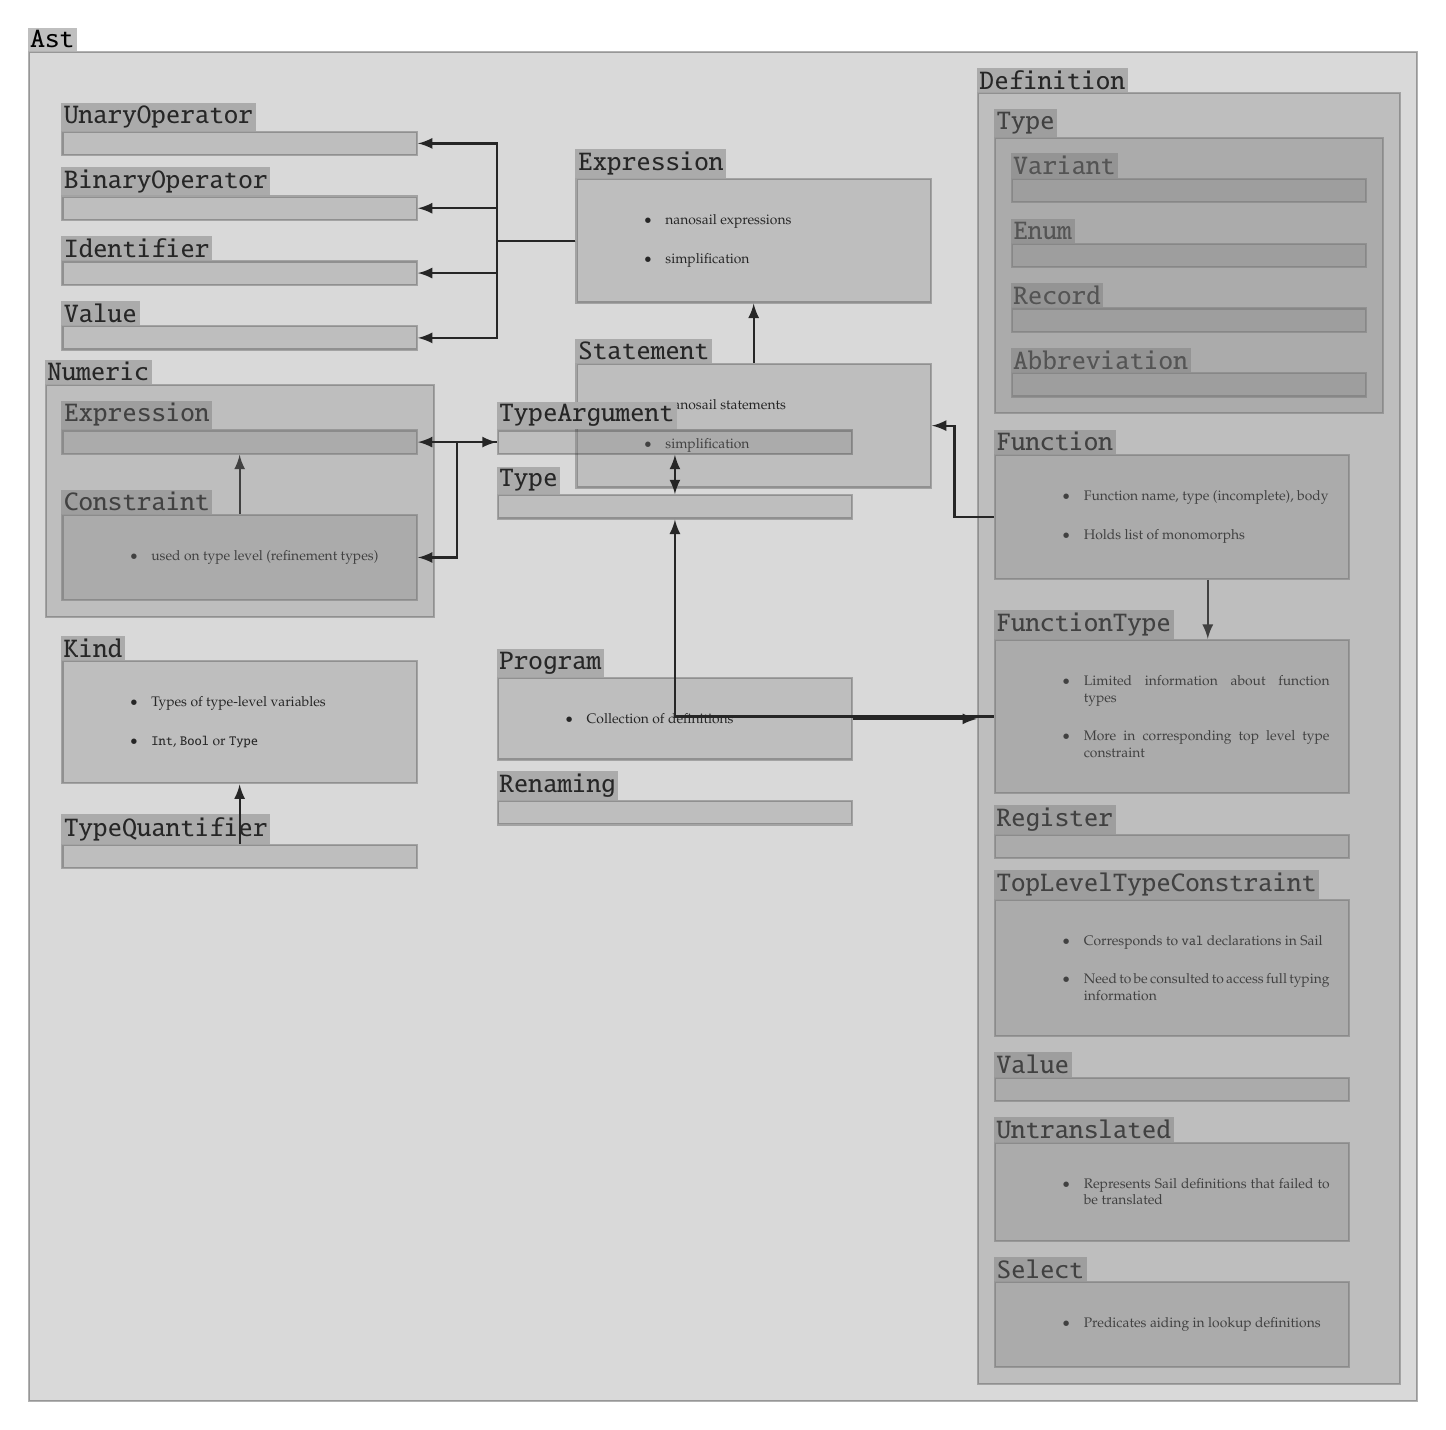
\begin{tikzpicture}[
    module box/.style={thick,draw,minimum width=4.5cm,inner sep=2pt,fill=gray,opacity=0.3,text opacity=1},
    module tag/.style={fill=gray!50,line width=0pt,inner sep=1pt},
    module group/.style={inner sep=0mm,line width=0pt},
    dependency/.style={-latex,thick},
    bidirectional dependency/.style={dependency,latex-latex},
  ]

  \module[id=ast-unaryoperator,name=UnaryOperator,at={(0,0)},submodule of=ast]{ }
  \module[id=ast-binaryoperator,name=BinaryOperator,below last,submodule of=ast]{}
  \module[id=ast-identifier,name=Identifier,below last,submodule of=ast]{}
  \module[id=ast-value,name=Value,below last,submodule of=ast]{}

  \coordinate (midpoint) at ($ (ast-unaryoperator--box.east) ! 0.5 ! (ast-value--box.east) $);

  \module[id=ast-expression,name=Expression,at={($ (midpoint) + (2,0) $)},box/.style={anchor=west},submodule of=ast]{
    \begin{itemize}
      \item nanosail expressions
      \item simplification
    \end{itemize}
  }

  \foreach \m in {ast-unaryoperator,ast-binaryoperator,ast-value,ast-identifier} {
    \draw[dependency] (ast-expression--box.west) -- +(-1,0) |- (\m--box.east);
  }

  \module[id=ast-statement,name=Statement,below last=0.75,submodule of=ast]{
    \begin{itemize}
      \item nanosail statements
      \item simplification
    \end{itemize}
  }
  \draw[dependency] (ast-statement--box.north) -- (ast-expression--box.south);


  \module[id=ast-numeric-expression,name=Expression,at={($ (ast-value.south west) + (0,-1) $)},submodule of=ast-numeric]{}
  \module[id=ast-numeric-constraint,name=Constraint,at={($ (ast-numeric-expression.south west) + (0,-0.75) $)},submodule of=ast-numeric]{
    \begin{itemize}
      \item used on type level (refinement types)
    \end{itemize}
  }
  \draw[dependency] (ast-numeric-constraint--box) -- (ast-numeric-expression--box);
  \supermodule{id=ast-numeric,name=Numeric,submodule of=ast}

  \module[id=ast-typeargument,name=TypeArgument,at={($ (ast-numeric-expression--box.north east) + (1,0) $)},submodule of=ast]{}
  \module[id=ast-type,name=Type,below last,submodule of=ast]{}
  \draw[bidirectional dependency] (ast-type--box.north) -- (ast-typeargument--box.south);
  \draw[dependency] (ast-typeargument--box.west) -- (ast-numeric-expression--box.east);
  \draw[bidirectional dependency] (ast-typeargument--box.west) -- +(-0.5,0) |- (ast-numeric-constraint--box.east);

  
  \module[id=ast-kind,name=Kind,submodule of=ast,below at={ast-numeric-constraint}{0.75}]{
    \begin{itemize}
      \item Types of type-level variables
      \item \texttt{Int}, \texttt{Bool} or \texttt{Type}
    \end{itemize}
  }
  \module[id=ast-typequantifier,name=TypeQuantifier,below last=0.75,submodule of=ast]{}
  \draw[dependency] (ast-typequantifier--box.north) -- (ast-kind--box.south);

  \module[id=ast-definition-variant,name=Variant,at={($ (ast-expression--box.north east) + (1,0) $)},submodule of=ast-definition-type]{}
  \module[id=ast-definition-enum,name=Enum,below last,submodule of=ast-definition-type]{}
  \module[id=ast-definition-record,name=Record,below last,submodule of=ast-definition-type]{}
  \module[id=ast-definition-abbreviation,name=Abbreviation,below last,submodule of=ast-definition-type]{}
  \supermodule{id=ast-definition-type,name=Type,submodule of=ast-definition}
  
  \module[id=ast-definition-function,name=Function,below=ast-definition-type,submodule of=ast-definition]{
    \begin{itemize}
      \item Function name, type (incomplete), body
      \item Holds list of monomorphs
    \end{itemize}
  }
  \module[id=ast-definition-functiontype,name=FunctionType,below last=0.75,submodule of=ast-definition]{
    \begin{itemize}
      \item Limited information about function types
      \item More in corresponding top level type constraint
    \end{itemize}
  }
  \coordinate (temp) at ($ (ast-definition-function--box.south west) ! 0.6 ! (ast-definition-function--box.south east) $);
  \draw[dependency] (temp) -- (temp |- ast-definition-functiontype--box.north);
  
  \module[id=ast-definition-register,name=Register,below last,submodule of=ast-definition]{}
  \module[id=ast-definition-topleveltypeconstraint,name=TopLevelTypeConstraint,below last,submodule of=ast-definition]{
    \begin{itemize}
      \item Corresponds to \texttt{val} declarations in Sail
      \item Need to be consulted to access full typing information
    \end{itemize}
  }
  \module[id=ast-definition-value,name=Value,below last,submodule of=ast-definition]{}
  \module[id=ast-definition-untranslated,name=Untranslated,below last,submodule of=ast-definition]{
    \begin{itemize}
      \item Represents Sail definitions that failed to be translated
    \end{itemize}
  }
  \module[id=ast-definition-select,name=Select,below last,submodule of=ast-definition]{
    \begin{itemize}
      \item Predicates aiding in lookup definitions
    \end{itemize}
  }
  \supermodule{id=ast-definition,name=Definition,below=ast-statement,submodule of=ast}
  
  \module[id=ast-program,name=Program,below at={ast-type}{2},submodule of=ast]{
    \begin{itemize}
      \item Collection of definitions
    \end{itemize}
  }
  \module[id=ast-renaming,name=Renaming,below last,submodule of=ast]{}

  \draw[dependency] (ast-program--box.east) -- (ast-program--box.east -| ast-definition.west);
  \draw[dependency] (ast-definition-function--box.west) -- +(-0.5,0) |- (ast-statement--box);
  \draw[dependency] (ast-definition-functiontype--box.west) -| (ast-type--box.south);
  
  \supermodule{id=ast,name=Ast}


\end{tikzpicture}

\end{document}